
%==================want_intro.tex=================
\section{Introduction}
\label{section:intro}

WanT is an open-source, GNU General Public License suite of codes that
provides an integrated approach for the study of coherent electronic
transport in low-dimensional, extended nanostructures. The core
methodology combines state-of-the-art Density Functional Theory (DFT),
plane-wave, norm-conserving pseudopotentials calculations with a Green's
functions method based on the Landauer formalism to describe quantum
conductance. The essential connection between the two, and a crucial step
in the calculation, is the use of the maximally-localized Wannier
function representation to introduce naturally the ground-state
electronic structure into the lattice Green's function approach at the
basis of the evaluation of the quantum conductance. Moreover, the
knowledge of the Wannier functions of the system allows the direct link
between the electronic transport properties of the device with the nature
of the chemical bonds, providing insight onto the mechanisms that govern
electron flow at the nanoscale.


We have tried to make this document complete and easy to understand as
well
as WanT itself easy to install and run.
We welcome any suggestion for improving the documentation and code
itself.

\subsection{Theoretical background - Quantum transport}

Calculations of the quantum conductance are based on a recently
developed efficient method for evaluating quantum transport in
extended systems.~\cite{marco,marco1,marco2} This method is applicable
to any Hamiltonian that can be expanded within a localized-orbital
basis and can be used as a general theoretical scheme for the
computation and analysis of the electrical properties of
nanostructures.

\subsubsection{Electron transmission and Green's functions}

Let us consider a system composed of a conductor, $C$, connected
to two semi-infinite leads, $R$ and $L$, as in Fig. \ref{fig:LCR}.
A fundamental result in the theory of electronic transport is that
the conductance through a region of interacting electrons (the $C$
region in Fig. \ref{fig:LCR}) is related to the scattering
properties of the region itself via the Landauer formula
\cite{Landauer}
\begin{equation}
{\mathcal C} = {2 e^2 \over h} {\mathcal T},
\end{equation}
where ${\mathcal T}$ is the transmission function and ${\mathcal
C}$ is the conductance. The former represents the probability that
an electron injected at one end of the conductor will transmit to
the other end. In principle, we can compute the transmission
function for a coherent conductor\footnote{A conductor is said to
be coherent if it can be characterized by a transmission matrix
that relates each of the outgoing wave amplitudes to the incoming
wave amplitudes at a given energy} starting from the knowledge of
the scattering matrix, $S$. The latter is the mathematical
quantity that describes the response at one lead due an excitation
at another. In principle, the scattering matrix can be uniquely
computed from the solution of the Schroedinger equation and would
suffice to describe the transport processes we are interested in
this work. However, it is a general result of conductance theory
that the elements of the S-matrix can be expressed in terms of the
Green's function of the conductor \cite{Datta,FisherLee,Meir}
which, in practice, can be sometimes simpler to compute.

Let us consider a physical system represented by an Hamiltonian
$H$. Its Green's function for an energy $E$ is defined by the
equation
\begin{equation}
(E\pm i\eta-H)G(\br,\br^{'})=\delta(\br,\br^{'})
\end{equation}
where $i\eta>0$ is an infinitesimal imaginary part added to the
energy to incorporate the boundary conditions into the equation.
The solution with $+$ sign is the retarded Green's function $G^r$,
while the solution with $-$ sign is called advanced Green's
function $G^a$. The transmission function can then be expressed in
terms of the Green's functions of the conductors and the coupling
of the conductor to the leads in a simple manner \cite[see][p.141
and ff.]{Datta}

\begin{equation}
{\mathcal T} = {\rm Tr}(\Gamma_L G_C^r \Gamma_R G_C^a),
\label{eq:T}
\end{equation}


where $G_C^{\{r,a\}}$ are the retarded and advanced Green's
functions of the conductor, and $\Gamma_{\{L,R\}}$ are functions
that describe the coupling of the conductor to the leads.

In the following we are going to restrict the discussion to
discrete systems that we can describe by ordinary matrix algebra.
More precisely, we are going to work with matrices representing a
physical system in the basis of localized electronic orbitals
centered on the atoms constituting the system. It includes in
particular the tight-binding model.

For a discrete media, the Green's function is then the solution of
a matrix equation
\begin{equation}
(\epsilon - H)G = I \label{green}
\end{equation}
where $\epsilon = E\pm{\rm i}\eta$ with $\eta$ arbitrarily small
and $I$ is the identity matrix. To simplify the notations, we drop
the exponent $\{a,r\}$ referring to advanced and retarded
functions when implicitly defined by $\epsilon$. For an open
system, consisting of a conductor and two semi-infinite leads (see
Fig. \ref{fig:LCR}), the above Green's function can be partitioned
into sub-matrices that correspond to the individual subsystems

\begin{equation}
\left(
\begin{array}{lll}
g_L� & g_{LC} &� g_{LCR}\\
g_{CL} & G_C & g_{CR} \\
g_{LRC} & g_{RC} & g_R
\end{array}
\right) = \left(
\begin{array}{ccc}
(\epsilon -h_L) & -h_{LC} & 0\\
-h_{LC}^\cc & (\epsilon -H_C) & -h_{CR}\\
0 & -h_{CR}^\cc & (\epsilon -h_R)
\end{array}
\right)^{-1}, \label{condmatr}
\end {equation}
where the matrix $(\epsilon -H_C)$ represents the finite
``isolated'' conductor (with no coupling elements to the leads),
$(\epsilon -h_{\{R,L\}})$ represent the semi-infinite leads, and
$h_{CR}$ and $h_{LC}$ are the coupling matrices between the
conductor and the leads, and $h^\cc$ denotes the familiar
conjugate transpose of $h$. As a convention, we use lower case
letters for (semi-)infinite matrices and upper case for finite
dimension matrices. In Eq.(\ref{condmatr}) we have made the
assumption that there is no direct interaction between the left
and right leads. From this equation it is straightforward to
obtain an explicit expression for $G_C$\cite{Datta}
\begin{equation}

G_C = (\epsilon -H_C -\Sigma_L -\Sigma_R)^{-1} \label{gconduct}
\end{equation}
where the finite dimension matrices
\begin{equation}
\Sigma_{L} = h_{LC}^\cc (\epsilon -h_L)^{-1} h_{LC}, \;\;\;\;
\Sigma_R = h_{RC} (\epsilon -h_R)^{-1} h_{RC}^\cc
\end{equation}
are defined as the self-energy terms due to the semi-infinite
leads. The self-energy terms can be viewed as effective
Hamiltonians that arise from the coupling of the conductor with
the leads. The coupling functions $\Gamma_{\{L,R\}}$ can then be
obtained as\cite{Datta}
\begin{equation}
\Gamma_{\{L,R\}} = {\rm i}[\Sigma_{\{L,R\}}^r -
\Sigma_{\{L,R\}}^a], \label{eq:gamma}
\end{equation}

where the advanced self-energy $\Sigma_{\{L,R\}}^a$ is the
Hermitian conjugate of the retarded self-energy
$\Sigma_{\{L,R\}}^r$. The core of the problem lies in the
calculation of the self-energies of the semi-infinite leads.


\begin{figure}
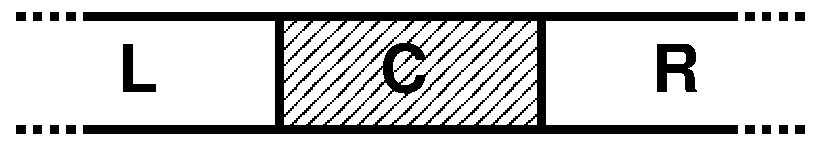
\includegraphics[width=8cm]{fig1.eps}
\caption{A conductor described by the Hamiltonian $H_C$, connected
to two semi-infinite leads $L$ and $R$, through the coupling
matrices $h_{LC}$ and $h_{CR}$.} \label{fig:LCR}
\end{figure}

It is well known that any solid (or surface) can be viewed as an
infinite (semi-infinite in the case of surfaces) stack of
principal layers with nearest-neighbor interactions
\cite{Joannopoulos1,Joannopoulos2}. This corresponds to
transforming the original system into a linear chain of principal
layers. For a lead-conductor-lead system, the conductor can be
considered as one principal layer sandwiched between two
semi-infinite stacks of principal layers. The next three sections
are devoted to the computation of the self-energies using the
principal layers approach for different geometries.

%%%%%%%%%%%%%%%%%%%%%%%%%%%%%%%%%%%%%%%%%%%%%%%%%%%%%%%%%%%%%%%%%%%

\subsubsection{Transmission through a bulk system.} \label{ss:bulk}

Within the principal layer approach, the matrix elements of
Eq.(\ref{green}) between layer orbitals yield a series of matrix
equations for the Green's functions

%yes

\begin{equation}
\begin{array}{ccl}
(\epsilon -H_{00}) G_{00} & = & I + H_{01}G_{10}\\
(\epsilon -H_{00}) G_{10} & = & H_{01}^\cc G_{00} + H_{01}G_{20}\\
\dots\\
(\epsilon -H_{00}) G_{n0} & = & H_{01}^\cc G_{n-1,0} +
H_{01}G_{n+1,0}
\end{array}
\label{serie}
\end{equation}

where the finite dimension matrices $H_{nm}$ and $G_{nm}$ are
formed by the matrix elements of the Hamiltonian and Green's
function between the layer orbitals. We assume that in a bulk
system $H_{00}=H_{11}=\dots$ and $H_{01}=H_{12}=\dots$. Following
\cite{LopezSancho1,LopezSancho2}, this chain can be transformed in
order to express the Green's function of an individual layer in
terms of the Green's function of the preceding (or following) one.
This is done via the introduction of the transfer matrices $T$ and
$\overline{T}$, defined such that
$$G_{10}=TG_{00}$$
and
$$G_{00}=\overline{T}G_{10}.$$
Using these definitions, we can write the bulk Green's function as
\cite{Garcia2}
\begin{equation}
\label{eq:GT} G(E) = (\epsilon - H_{00} - H_{01}T
-H_{01}^\cc\overline{T})^{-1}.
\end{equation}

The transfer matrix can be easily computed from the Hamiltonian
matrix elements via an iterative procedure, as outlined in
\cite{LopezSancho1,LopezSancho2}. In particular $T$ and $\overline
T$ can be written as
\[
\begin{array}{c}
T = t_0 + \tilde{t}_0t_1 + \tilde{t}_0\tilde{t}_1t_2+\ldots+
\tilde{t}_0\tilde{t}_1\tilde{t}_2\cdots t_n \\
\overline T = \tilde{t}_0 + t_0\tilde{t}_1 +t_0t_1\tilde{t}_2
+\ldots+ t_0t_1t_2\cdots\tilde{t}_n
\end{array}
\]
where $t_i$ and $\tilde{t}_i$ are defined via the recursion
formulas
\[
\begin{array}{l}
t_i = (I -t_{i-1}\tilde{t}_{i-1} - \tilde{t}_{i-1}t_{i-1})^{-1}
t_{i-1}^2, \\
\tilde{t}_i = (I -t_{i-1}\tilde{t}_{i-1} -
\tilde{t}_{i-1}t_{i-1})^{-1} \tilde{t}_{i-1}^2
\end{array}
\]
and
\[
\begin{array}{l}
t_0 = (\epsilon - H_{00})^{-1} H_{01}^\cc,\\
\tilde{t}_0 = (\epsilon - H_{00})^{-1} H_{01}.
\end{array}
\]
The process is repeated until $t_n,\tilde{t}_n \le \delta$ with
$\delta$ arbitrarily small. Usually no more than 5 or 6 terms are
required to converge the above sum.


If we compare Eq.(\ref{eq:GT}) with Eq. (\ref{gconduct}), in the
hypothesis of leads and conductors being of the same material
(bulk conductivity), we can identify one principal layer of the
bulk system with the conductor $C$, so that $H_{00}\equiv H_C$. In
particular, by comparing with Eq.(\ref{gconduct}), we obtain the
expression of the self-energies of the conductor-leads system
\begin{equation}

\Sigma_L = H_{01}^\cc \overline T, \;\;\;\;\; \Sigma_R = H_{01} T.

\label{eq:sigmabulk}

\end{equation}



The coupling functions are then obtained from the sole knowledge

of the transfer matrices and the coupling Hamiltonian matrix

elements: $\Gamma_L=-{\rm Im}(H_{01}^\cc \overline T)$ and

$\Gamma_R=-{\rm Im}(H_{01} \overline T)$\cite{nardelli1999_1270}.



\begin{remark}

In the application of the Landauer formula, it is customary to

compute the transmission probability from one lead to the other

assuming that the leads are connected to a reflectionless contact

whose electron energy distribution is known\cite[see for

instance][p. 59 and ff.]{Datta}.

\end{remark}



%%%%%%%%%%%%%%%%%%%%%%%%%%%%%%%%%%%%%%%%%%%%%%%%%%%%%%%%%%%%%%%%%%%%

\subsubsection{Transmission through an interface.} \label{ss:interf}



The procedure outlined above can also be applied in the case of

electron transmission through an interface between two different

media $A$ and $B$. To study this case we make use of the Surface

Green's Function Matching (SGFM) theory, pioneered by

\cite{Garcia1,Garcia2}.



We have to compute the Green's function $G_I$, where the subscript

$I$ refers to the interface region composed of two principal

layers

--- one in each media --- (see Fig.\ref{fig:interface}). Using the SGFM

method, $G_I$ is calculated from the bulk Green's function of the

isolated systems, $G_A$ and $G_B$, and the coupling between the

two principal layers at the two sides of the interface, $H_{AB}$

and $H_{BA}$. Via the calculation of the transmitted and reflected

amplitudes of an elementary excitation that propagates from medium

A to medium B, it can be shown that the interface Green's function

obeys the following equation\cite[Ch.4]{Garcia2}

\begin{equation}

G_I= \left(

\begin{array}{cc}

G_{AA} & G_{AB}\\

G_{BA} & G_{BB}\\

\end{array}

\right)~=~ \left(

\begin{array}{cc}

\epsilon -H^A_{00} - (H^A_{01})^\cc \overline T & -H_{AB}\\

-H_{BA} & \epsilon -H^B_{00} - H^B_{01} T \\

\end{array}

\right)^{-1}. \label{secular}

\end{equation}



\begin{figure}

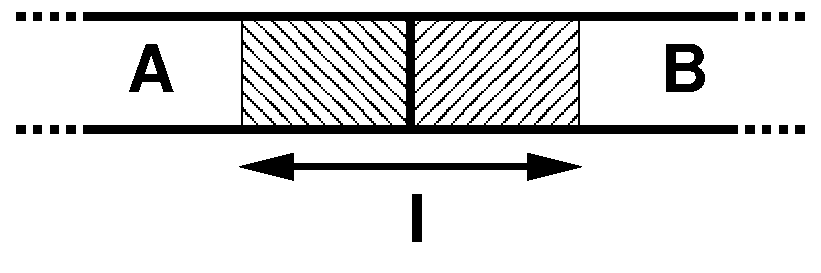
\includegraphics[width=8cm]{fig2.eps}

\caption{Sketch of a system containing an interface between two

media A and B. $I$ is the interface region for which we need to

compute the Green's function $G_I$. $I$ is composed of two

principal layers, one in each side of the interface (dashed area).

} \label{fig:interface}

\end{figure}



Once the interface Green's function is known, we can compute the

transmission function in terms of block super-matrices

\[

{\mathcal T}(E) = {\rm Tr}(\Gamma_A G_{AB}^r \Gamma_B G_{BA}^a)

\]

with $\Gamma_{\{A,B\}} = {\rm i}[\Sigma_{\{A,B\}}^r -

\Sigma_{\{A,B\}}^a]$, $\Sigma_{\{A,B\}}$ given by the analogous of

Eq.(\ref{eq:sigmabulk}) for the two semi-infinite sections, and

$G_{BA}^a = (G_{AB}^r)^\cc$ \cite{nardelli1999_1270}.



%%%%%%%%%%%%%%%%%%%%%%%%%%%%%%%%%%%%%%%%%%%%%%%%%%%%%%%%%%%%%%%

\subsubsection{Transmission through a left lead-conductor-right lead

(LCR) system.} \label{ss:LCR}



Within the SGFM framework, the approach described in the previous

section can be extended to the case of multiple interfaces and

superlattices \cite{Garcia1,Garcia2} with little complication.

For the calculation of conductances in realistic experimental

geometry, the method can be expanded to the general configuration

of a Left-lead-Conductor-Right-lead (LCR) systems --- as displayed

in Fig.\ref{fig:LCR}. In the language of block matrices and

principal layers, outlined in the previous sections, the LCR

Green's function obeys the following secular equation



\begin{eqnarray}

\nonumber G_{LCR}&=& \left(

\begin{array}{ccc}

G_{L} & G_{LC} & G_{LR}\\

G_{CL} & G_{C} & G_{CR}\\

G_{RL} & G_{RC} & G_{R}\\

\end{array}

\right) \\ &=& \left(

\begin{array}{ccc}

\epsilon -H^L_{00} - (H^L_{01})^\cc \overline T & -H_{LC} & 0\\

-H_{CL} & \epsilon -H_{C} & -H_{CR}\\

0 & -H_{RC} & \epsilon -H^R_{00} - H^R_{01} T \\

\end{array}

\right)^{-1}. \label{secular1}

\end{eqnarray}

where $H_{nm}^{\{L,R\}}$ are the block matrices of the Hamiltonian

between the layer orbitals in the left and right leads

respectively, and $T_{\{L,R\}}$ and $\overline{T}_{\{L,R\}}$ are

the appropriate transfer matrices. The latter are easily computed

from the Hamiltonian matrix elements via the iterative procedure

already described in the bulk case (Sec.\ref{ss:bulk}).

Correspondingly, $H_{LC}$ and $H_{CR}$ are the coupling matrices

between the conductor and the leads principal layers in contact

with the conductor.



As in Sec.\ref{se:trans}, it is straightfroward to obtain in the form

of Eq.(\ref{gconduct}), $G_C = (\epsilon -H_C -\Sigma_L

-\Sigma_R)^{-1}$, where $\Sigma_{L}$ and $\Sigma_R$ are the

self-energy terms due to the semi-infinite leads, and

identify\cite{nardelli1999_1252}



\begin{equation}

\begin{array}{ccl}

\Sigma_L & = & H_{LC}^\cc (\epsilon -H_{00}^L-(H_{01}^L)^\cc

\overline T_L)^{-1} H_{LC},\\ \Sigma_R & = & H_{CR} (\epsilon

-H_{00}^R-H_{01}^R T_R)^{-1} H_{CR}^\cc.\\

\end{array}

\end{equation}



The transmission function in the LCR geometry can then be derived

from Eq.(\ref{eq:T}) and (\ref{eq:gamma}).



\begin{remark}

The knowledge of the conductor's Green's function $G_C$ gives also

direct information on the electronic spectrum of the system via

the spectral density of electronic states

$$

N(E)=-(1/\pi) {\rm Im}[{\rm Tr}(G_C(E))].

$$

\end{remark}



\begin{remark}

We have assumed a truly one-dimensional chain of principal layers,

which is physical only for systems like nanotubes or quantum wires

that have a definite quasi-one-dimensional character. The

extension to a truly three-dimensional case is straightforward

using Bloch functions in the directions perpendicular to the

conduction. The introduction of the principal layer concept

implies that along the direction of the layer expansion the system

is described by an infinite set of $k_\bot$ while $k_\|$ is still

a good quantum number for the problem. The above procedure

effectively reduces the three-dimensional system to a set of

non-interacting linear-chains, one for each $k_\|$

\cite{Joannopoulos1,Joannopoulos2}. We can then use the usual

$k$-point summation techniques to evaluate, for instance, the

quantum conductance

$$

T(E) = \sum_{k_\|} w_{k_\|}T_{k_\|}(E)

$$

where $w_{k_\|}$ are the relative weights of the different

$k_\|$'s in the irreducible wedge of the surface Brillouin zone

\cite{Baldereschi:1}.



\end{remark}


\subsection {Teoretical background - Maximally-localized Wannier
functions}

Bloch orbitals cannot be used directly to evaluate electronic
transport with the method outlined in
Sec. \ref{tbmethod}. As we have pointed out,
the quantum conductance is computed starting from the knowledge of
the lattice Green's
function, whose calculation relies on a localized orbital
representation of the electronic states in real space. Bloch orbitals,
that are intrinsically delocalized, have to be transformed into {\em
localized} functions in order to construct the sparse, short-ranged
matrix
elements of the Hamiltonian.
The core of our proposed methodology
is to use maximally-localized WFs for the system considered. These
are the most natural choice for a set of localized orbitals
that still span the same Hilbert space of the Hamiltonian
eigenfunctions, and they allow� to bridge plane-wave
electronic structure and lattice Green's function calculations in a
coherent fashion.
In the case of an isolated system the maximally-localized WFs
become Boys localized orbitals;~\cite{boys}
therefore, our procedure is not
tied to an extended-systems formulation, but can equally well
represent isolated molecules. (In addition,
the localization procedure is greatly simplified for the
case of large unit cells, when $\Gamma$-sampling only is used
\cite{Silvestrelli}).

A Wannier function $w_{n{\bf R}}({\bf r})$, labeled by the Bravais
lattice vector {\bf R}, is usually defined via a unitary transformation
of
the Bloch functions $\psi_{n{\bf k}}({\bf r})$ of the $n$th
band:
\begin{equation}
w_{n{\bf R}}({\bf r})=\frac{V}{(2\pi)^3}\int_{BZ}\psi_{n{\bf k}}({\bf r})
e^{-i{\bf k}\cdot{\bf R}} d^3k,
\label{wf}
\end{equation}
where V is the volume of the unit cell and the integration is performed
over
the entire Brillouin Zone.� It is easy to show that the WFs defined as
above form an orthonormal basis set, and that any two of them, for a
given
index $n$ and different ${\bf R}$ and ${\bf R^\prime}$, are just
translational images of each other.
Note that, as the ${\mathcal N}$ WFs
form a (continuous) linear combinations of Bloch functions with
different energies, they do not represent stationary states, but
still span exactly the same original Hilbert space.
The {\em ab-initio} eigenstates are well-defined, modulus an arbitrary
${\bf k}$-dependent phase factor; thus, the definition above
does not lead to a unique set of Wannier functions~\cite{kohn},
since the electronic structure problem is invariant for the
transformation
$\psi_{n{\bf k}} \leadsto e^{\phi_n({\bf k})} \psi_{n{\bf k}} $.
Besides this freedom in the choice of
phases $\phi_n({\bf k})$ for the Bloch functions,
there is a more comprehensive gauge freedom stemming from the fact that
the
many-body wavefunction is actually a Slater determinant: a unitary
transformation between orbitals will not change the manifold, and
will not change the total energy and the charge density of the system.
In all generality, starting with a set of ${\mathcal N}$ Bloch
functions with periodic parts $u_{n{\bf k}}$, we can constructs infinite
sets of ${\mathcal N}$ WFs displaying different spatial characteristics:
\begin{equation}
w_{n{\bf R}}({\bf r})=\frac{V}{(2\pi)^3}\int_{BZ}
\left[ \sum_m U_{mn}^{({\bf k})}
\psi_{m{\bf k}}({\bf r}) \right]
e^{-i{\bf k}\cdot{\bf R}} d^3k.
\label{u1}
\end{equation}
The unitary matrices $U^{({\bf k})}$ include also the gauge freedom
on phase factors afore mentioned.~\cite{nicola}

For our purposes, we need to transform the Bloch eigenstates
in WFs with the narrowest spatial distribution.� We
construct {\em maximally-localized WFs} using the
algorithm proposed by Marzari and
Vanderbilt.~\cite{nicola}� We define a {\em Spread Operator}
($\Omega$) as the sum of the second
moments of the Wannier functions corresponding to one choice of
translational lattice vector:
\begin{equation}
\Omega=\sum_n [\langle w_{n{\bf 0}} | r^2 | w_{n{\bf 0}} \rangle -
\langle w_{n{\bf 0}} | {\bf r} | w_{n{\bf 0}} \rangle^2] ,
\label{omega}
\end{equation}
where the sum is over the group of bands which spans the Hilbert space.
The value of the spread $\Omega$ depends on the choice of unitary
matrices
$U^{({\bf k})}$; thus� it is possible
to evolve any arbitrary set of $U^{({\bf k})}$ until the minimum
condition
\begin{equation}
\frac {\delta \Omega_{\bf k}}{\delta U^{({\bf k})}}=0
\label{minimo}
\end{equation}
is satisfied.
At the minimum, we obtain the matrices $(U^{({\bf k})})^{ML}$
that transform the first-principles
$\psi_{n{\bf k}}^{FP}({\bf
r})$ into the {\em maximally-localized WFs}
$w_{n{\bf R}}^{ML}({\bf r})$:
\begin{equation}
\begin{array}{lll}
\psi_{n{\bf k}}^{ML}({\bf r})&=&\sum_{m} (U_{mn}^{({\bf k})})^{ML}
\psi_{m{\bf k}}^{FP}({\bf r}),\\ \\ w_{n{\bf R}}^{ML}({\bf
r})&=&\frac{V}{(2\pi)^2} \int_{BZ}
\psi_{n{\bf k}}^{ML}({\bf r}) e^{-i{\bf k}\cdot{\bf R}} d{\bf k} .\\
\end{array}
\end{equation}

A useful feature of the method is that the only ingredients needed to
calculate the spread functional
$\Omega$ and to evolve the unitary matrices $U^{({\bf k})}$ are
the overlap matrix $M_{mn}^{({\bf k},{\bf b})}$
between the periodic part of the Bloch states at neighboring {\bf
k}-points:
\begin{equation}
M_{mn}^{({\bf k},{\bf b})}=\langle u_{m,{\bf k}} | u_{n,{\bf
k+b}}\rangle,
\label{m}
\end{equation}
where {\bf b} is the vector that links neighboring {\bf k}-points
in the discretized BZ integrals.~\cite{note_ref}

It is important to notice that whenever a Born-von Karman discretization
of the Brillouin Zone is introduced, even the above-mentioned WFs are not
truly
localized, but will be periodic in real-space, with a {\em
superperiodicity}
determined by the BZ discretization. The truly isolated limit is
recovered only in the case of continuous BZ integrations.
This is easily seen remembering that
$ \psi_{n{\bf k}}({\bf r})= u_{n{\bf k}}({\bf r})
e^{i{\bf k}\cdot{\bf r}} $, and $� u_{n{\bf k}}({\bf r}) $ has the
periodicity of the direct lattice; thus the phase factors
$ e^{i{\bf k}\cdot{\bf r}}� $ determine the
{\em superperiodicity} of the $ \psi_{n{\bf k}} $ themselves.
In the standard language of electronic-structure
calculations, if the $ \psi_{n{\bf k}} $ have ${\bf k}$'s that are
restricted to
a uniform Monkhorst-Pack mesh, they will all be periodic with a
wavelength
inversely proportional to the spacing of the mesh; this periodicity is
consequently inherited by the WFs.
For $\mathcal N$ {\bf k}-points along a
direction of the BZ, the WFs will repeat along the corresponding
direction every $\mathcal N$ cells;
therefore a mesh of {\bf k}-points needs to be dense enough to assure
that adjacent replicas of the WFs do not overlap.\\

The method described above works properly in the case of {\em isolated
groups} of bands.~\cite{note1}� On the other hand to study quantum
conductance in extended systems we often need to compute
WFs for a subset of energy bands that are entangled or mixed
with other bands.� Most often we are interested in the
states that lie in the vicinity of the Fermi level of a conductor
in a restricted energy range.� Since the unitary transformations
$U^{({\bf k})}$ mix energy bands at each {\bf k}-point,
any arbitrary choice of states inside a prescribed
window will affect the localization properties of WFs unless
energy gaps
effectively separate the manifold of interest from higher and lower
bands.
This problem has been solved by Souza, Marzari, and Vanderbilt,
introducing
an additional disentanglement procedure~\cite{ivo2} that automatically
extracts the best possible manifold of a given dimension from the states
falling in a predefined energy window. This is the generalization to
{\em entangled} or metallic cases of the maximally-localized WF
formulation.� The procedure relies on minimizing the
subspace dispersion across the Brillouin Zone, and effectively
extracts the bands of interest from the overall band structure.�
In practice, first we select a desired number of bands in an energy
window;� then
we determine the optimally-connected subspace that can be
extracted from that band structure; and finally we proceed with
a standard localization procedure inside the selected subspace, using
the same kind of spread functional $\Omega$ and of unitary matrices
$U^{({\bf k})}_{mn}$.
The resulting orbitals have the same good localization properties, and
allow to apply our formalism to arbitrary systems, independently
of the insulating or metallic nature of the band manifold. It should
be stressed that the WFs obtained in the later case are not the WFs
of the occupied subspace (that would exhibit poor localization
properties), but
are those of a well connected, continuous subspace that in general will
contain both occupied and unoccupied Bloch functions.

In order to calculate the conductance according to the prescriptions
outlined
in Sec.~\ref{tbmethod}, we need as an input the matrix elements of the
Hamiltonian calculated on a localized basis: in our case, it is the
minimal basis of the maximally-localized WFs. The advantages of this
choice
are twofold: firstly, besides being a minimal basis, the WFs
span {\it exactly} the Hilbert space of an insulator and, with arbitrary
accuracy, of an entangled metallic system.
Secondly, their localization assures the choice of the system with the
smallest number
of atomic layers.
The Hamiltonian matrices ($H^{LR}_{mn}$,
$H_C$, $H_{LC}$, $H_{CR}$) can be formally obtained from the {\em on
site} ($H_{00}$) and {\em coupling} ($H_{01}$) matrices between {\em
principal layers}.� In our formalism, and assuming a BZ sampling fine
enough to eliminate the interaction with the periodic images, we
can simply compute these matrices from the
unitary matrix $U^{({\bf k})}$ obtained in the localization
procedure.~\cite{note2} By definition of energy eigenvalues
($\widetilde{\epsilon}_{m{\bf k}}$), the Hamiltonian matrix
$\widetilde{H}_{mn}({\bf k})= \widetilde{\epsilon}_{m{\bf k}}
\delta_{m,n}$, is diagonal in the basis of the Bloch eigenstates.� We
can calculate the Hamiltonian matrix in the rotated basis,
\begin{equation}
H^{(rot)}({\bf k})=(U^{({\bf k})})^{\dagger}\widetilde{H}({\bf
k})U^{({\bf k})}.
\label{rot}
\end{equation}
Next we Fourier transform $H^{(rot)}({\bf k})$ into a set of $N_{kp}$
Bravais lattice vectors {\bf R} within a Wigner-Seitz supercell
centered around {\bf R}=0 :
\begin{equation}
H^{(rot)}_{mn}({\bf R})=\frac{1}{N_{kp}} \sum_{\bf k}
e^{-i{\bf k}\cdot {\bf R}}H^{(rot)}_{mn}({\bf k})=\langle w_{m{\bf 0}}
| \widehat{H} | w_{n{\bf R}} \rangle,
\label{hrrot}
\end{equation}
where $N_{kp}$ derives from the folding of the uniform mesh of {\bf
k}-points in the BZ.� The term with {\bf R}=0 provides the {\em
on site} matrix $H_{00}=\langle w_{m{\bf 0}} | \widehat{H} | w_{n{\bf
0}}\rangle$, and the term {\bf R}=1 provides the {\em coupling} matrix
$H_{01}=\langle w_{m{\bf 0}} | \widehat{H} | w_{n{\bf 1}}\rangle$:
These are the only ingredients required for the evaluation of
the quantum conductance.

